% Based on the
% latex-beamer/latex-beamer/solutions/conference-talks/conference-ornate-20min.en.tex
% file
%Rob Lass <my name at google's free webmail domain>


\documentclass{beamer}

\usepackage{tabularx}

\newcommand{\bigsum}{\displaystyle\sum}
\newcommand{\fail}{\widetilde}

\def\reducify{
  \parindent 0pt
  \parskip   0pt
  \itemsep   0pt
  \topsep    0pt
  \parsep    0pt
}

\mode<presentation>
{
    \setbeamertemplate{background canvas}[vertical shading][bottom=yellow!10,top=blue!10]
	\usetheme[numbers]{Madrid}
	\setbeamercovered{invisible}
}

\usepackage{ulem}
\usepackage[english]{babel}

\usepackage[latin1]{inputenc}

\usepackage{times}
\usepackage{multirow}
\usepackage[T1]{fontenc}
\usepackage{xifthen}

\usepackage{tikz}
\usetikzlibrary{shapes,backgrounds,arrows,calc,fadings,decorations,shadows,decorations.markings}
\tikzfading[name=fade out,top color=transparent!0,bottom color=transparent!100]
\tikzfading[name=fade in,top color=transparent!100,bottom color=transparent!0]

\title[!is\_num(me)]
{Yes!  We're All Individuals!\\or The Importance of Context}

\author[Lass]
{Robert N. Lass}
\institute[Drexel \& AWeber]
{
AWeber Communications\\
Chalfont, PA\\
\&\\
Drexel University\\
Philadelphia, PA
}

\date[DataPhilly]
{April 14$^{th}$, 2014}
\begin{document}

\begin{frame}
\titlepage
\end{frame}

\section{Introduction}
\begin{frame}
    \frametitle{In the Beginning, There was Dice}
    \begin{columns}{}
        \begin{column}{0.5\textwidth}
            \begin{block}{}
                \begin{itemize}
                    \item Astragali (knuckle bones) is one of the world's
                        oldest known games.
                    \begin{itemize}
                        \item Appears in numerous ancient texts including the
                            Iliad, the Odyssey, and the bible.
                    \end{itemize}
                    \item The Greeks were pretty smart dudes and dudettes.  How
                        did they approach this game?
                \end{itemize}
            \end{block}
        \end{column}
        \begin{column}{0.5\textwidth}
            \begin{block}{}
                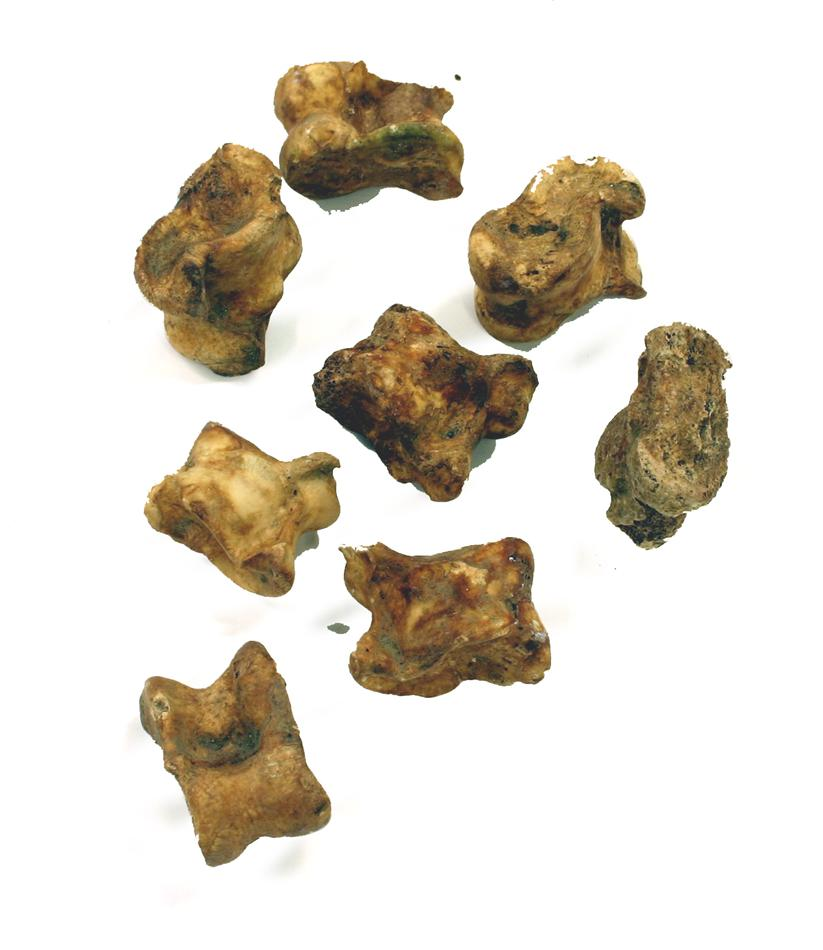
\includegraphics[width=0.5\hsize]{art/knucklebones.jpg}
                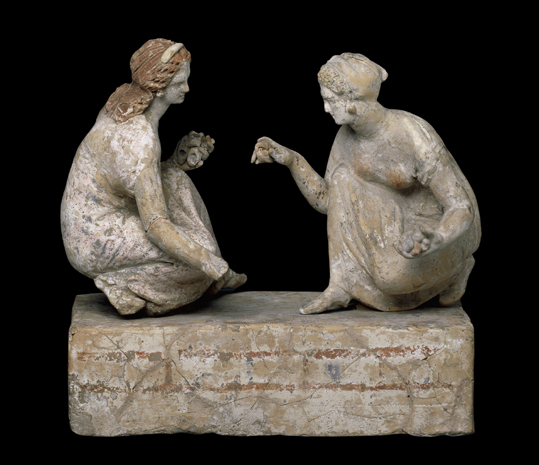
\includegraphics[width=0.8\hsize]{art/playing_knuckle_bones.jpg}
            \end{block}
        \end{column}
    \end{columns}
\end{frame}

%------------------------------------------------

\begin{frame}
    \frametitle{I Must be Certain!}
    \begin{columns}{}
        \begin{column}{0.75\textwidth}
            \begin{block}{}
                \begin{itemize}
                    \item The Greeks disregarded things that could not be
                        proven with absolute certainty.
                    \item Preferred oracles to philosophers for predicting the
                        future.
                    \item ``Gods'' or ``luck'' determine my fate at the
                        gambling table.
                    \item When analyzed using modern mathematics, the stakes in
                        their games of chance are senseless.
                \end{itemize}
            \end{block}
        \end{column}
        \begin{column}{0.25\textwidth}
            \begin{block}{}
                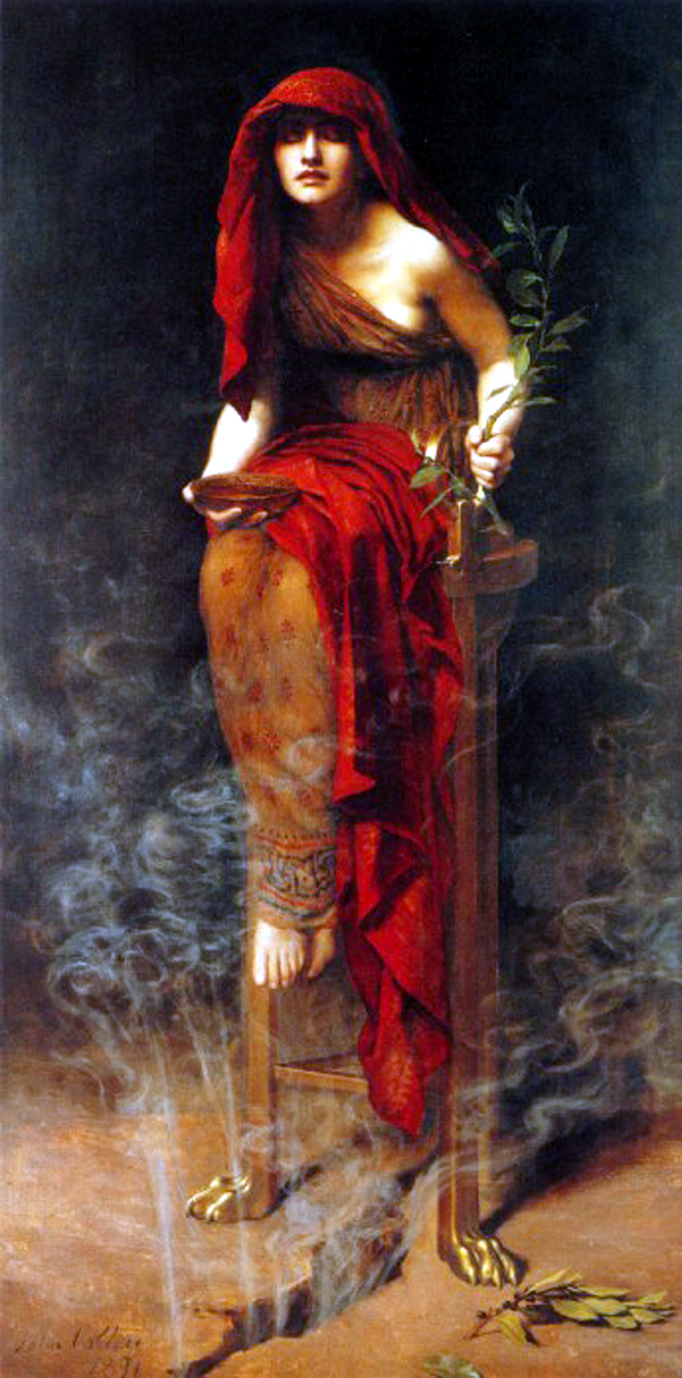
\includegraphics[width=\hsize]{art/priestess_of_delphi.jpg}
            \end{block}
        \end{column}
    \end{columns}
\end{frame}

%------------------------------------------------

\begin{frame}
\frametitle{The Most Important Man You Don't Know}
\textbf{Luca Pacioli}
\begin{itemize}
    \item Introduced double-entry bookkeeping to the West.
    \item<2-> Invented the \textit{Rule of 72}.
    \item<3-> Most importantly for us, he formalized games of chance
    mathematically.
    \item<4->Lived in the $15^{th}$ century.
\end{itemize}
\end{frame}

%------------------------------------------------

\begin{frame}
\frametitle{Gambling Scientifically}
\begin{itemize}
\item John Graunt publishes \underline{Natural and Political Observations} 
 \underline{Made upon the Bills of Mortality} in 1662.\pause
\item Many European cities used annuities to finance themselves.\pause
\item In 1540, London issued annuities that repaid the full purchase price in seven
years.\pause
\item In 1789, they did somewhat better, issuing annuities that took fourteen
years to pay out the original purchase price.\pause
\end{itemize}
\end{frame}

%------------------------------------------------

\begin{frame}
\frametitle{Risky Business}
\begin{itemize}
\item Private industry adapted the principles of using statistics to manage
risk much faster.
\item Lloyd's Coffee House founded in 1774 as a sailors' hangout\pause
\item Evolved into an insurance clearinghouse.\pause
\item Policies for ``house-breaking, highway robbery, death by gin
drinking, death of horses and assurance of female chastity.''\pause
\item Not insurance like in modern times:  it was a clearing house for
individuals taking either side of the ``bet''.
\end{itemize}
\end{frame}

%------------------------------------------------

\begin{frame}
\frametitle{Signet Bank}
\begin{itemize}
    \item<1->In the 1990s, Fairbanks and Morris wanted to predict
        profitability.
    \item<2->Had trouble selling this, but tiny Signet Bank took them on.
    \item<3->Problem:  No data.
    \item<4->Solution: Offer random terms to customers, to collect data.
    \item<5->Eventually became so profitable, the credit business was spun off.
    \item<6->The spin off is called ``Capital One''. 
\end{itemize}
\end{frame}

%------------------------------------------------

\section{Individuals are Not the Population}
\begin{frame}
	\frametitle{Insurance}
	\begin{itemize}
        \item<1->Prob/stat can be wildly successful in business.
        \item<2->22 yr old Porche-driver vs 45 yr old Camry-driver
        \item<3->Intuitively, this won't work for everyone.
    \end{itemize}
\end{frame}

%------------------------------------------------

\begin{frame}
	\frametitle{Estimating Age}
	\begin{itemize}
        \item \textit{Estimating Age, Gender, and Identity Using First Name
                Priors} by Gallagher and Chen
        \item Fuse name information with CV data algorithms.
        \item<2->I recently saw a talk where someone proposed using part of this.
    \end{itemize}
\end{frame}

%------------------------------------------------

\begin{frame}
	\frametitle{Genevieve}
    \begin{center}
        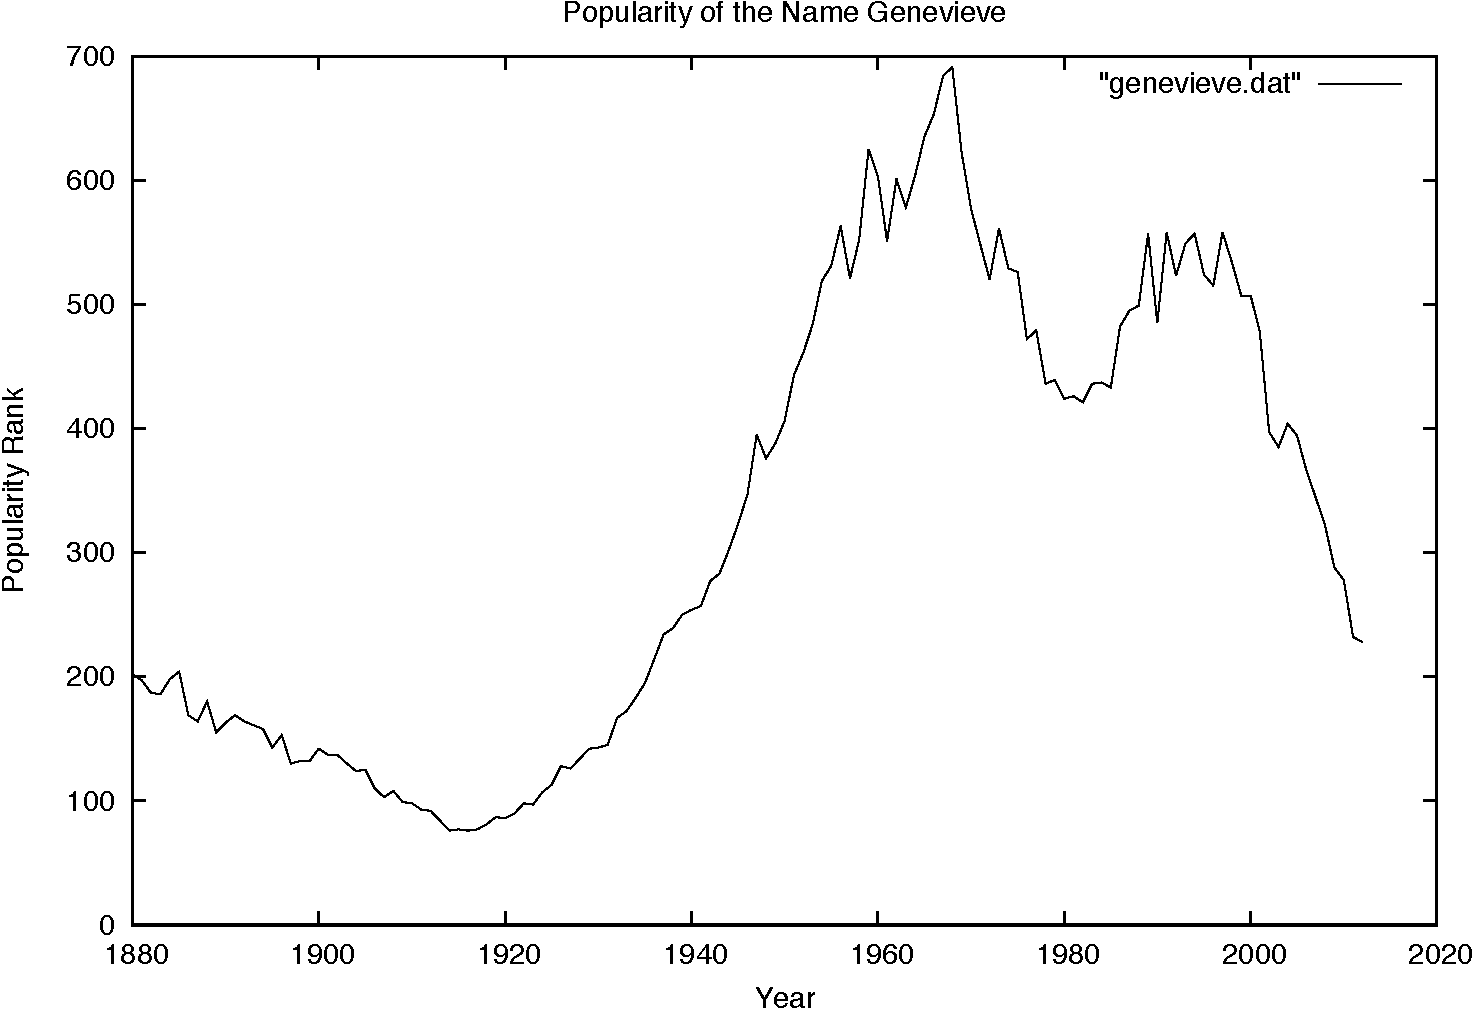
\includegraphics[width=0.8\hsize]{art/genevieveyears}
    \end{center}
\end{frame}

\begin{frame}
	\frametitle{Genevieve}
    \begin{center}
        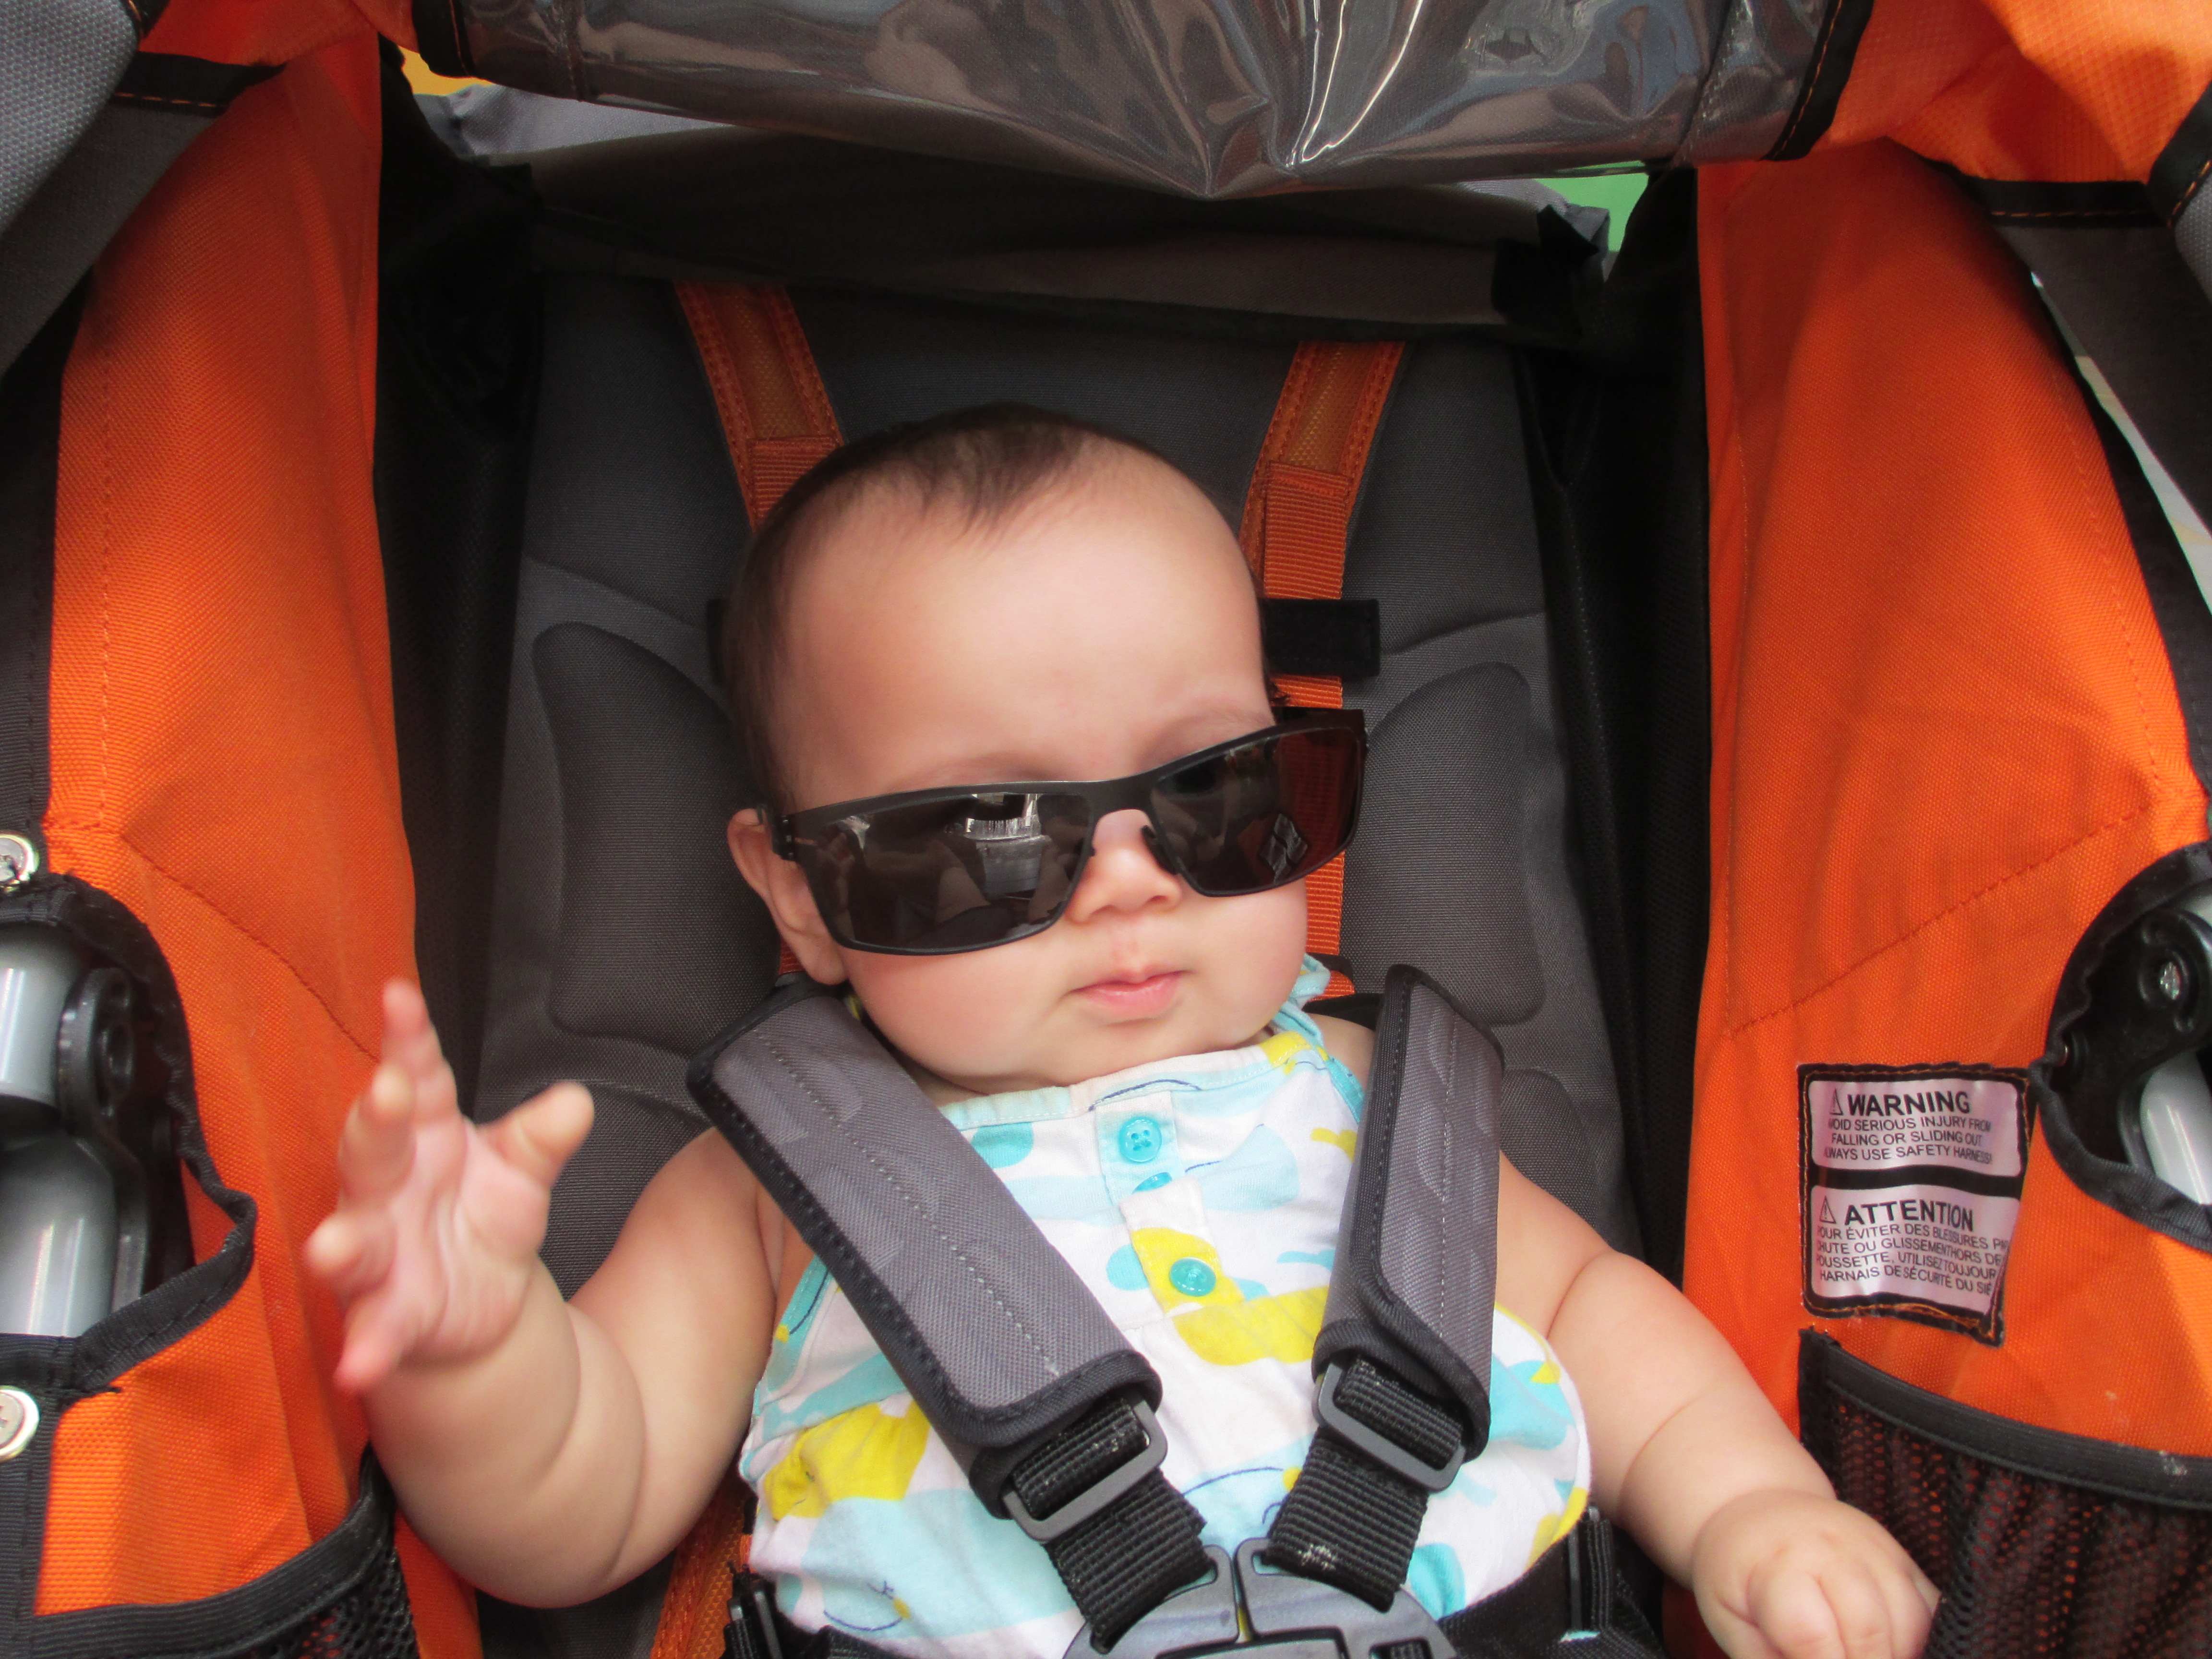
\includegraphics[width=0.8\hsize]{art/genevievedaughter}
    \end{center}
\end{frame}

%------------------------------------------------

\begin{frame}
\frametitle{Populations:  Sampled Statistics}
\begin{itemize}
    \item Total measurement of all individuals.
    \item Sampled statistics should be close \emph{if you have a
        representative sample}.
    \begin{itemize}
        \item That means if you take one sample, and then another sample, they
            should be similar.
    \end{itemize}
    \item An individual can never be a representative sample.
    \item You \emph{can} make probabilistic statements about individuals.
\end{itemize}
\end{frame}

%------------------------------------------------

\begin{frame}
	\frametitle{Genevieve}
    \begin{center}
        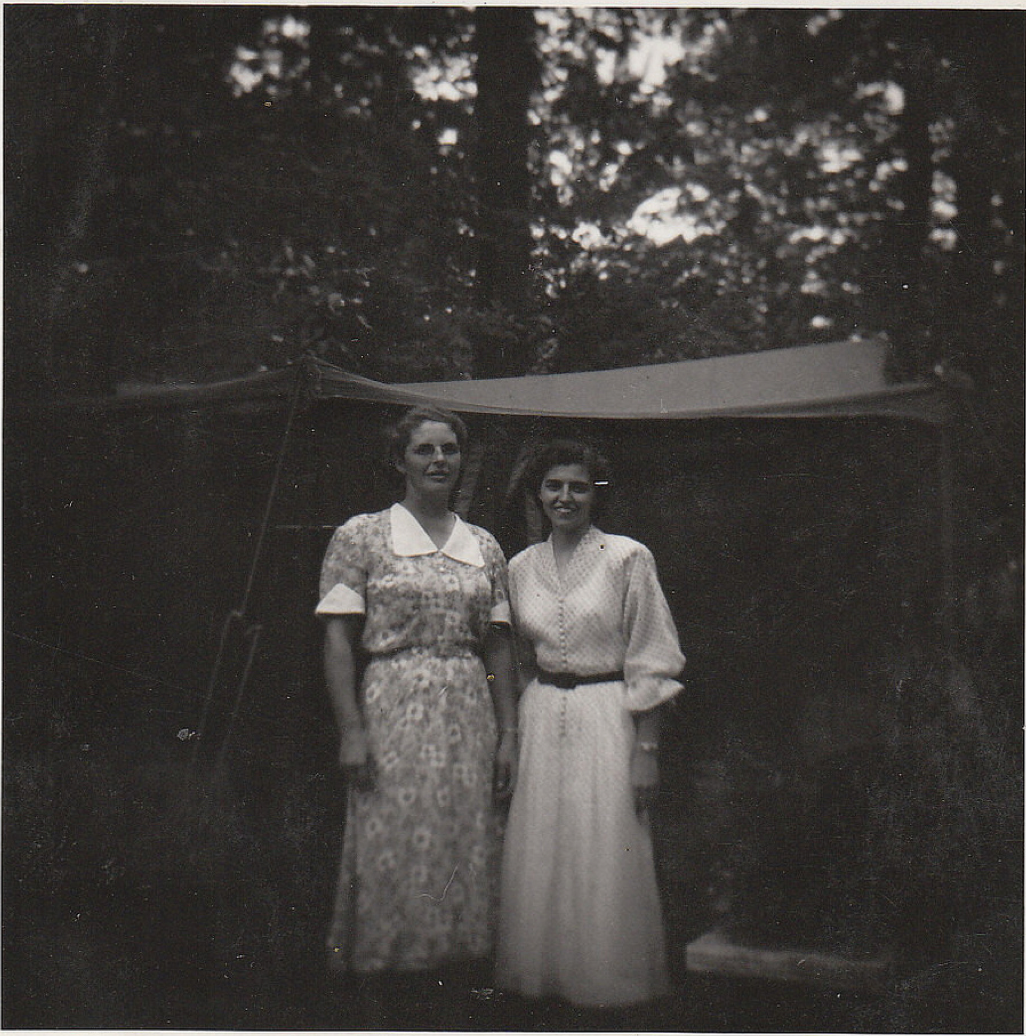
\includegraphics[width=0.5\hsize]{art/auntgenevieve}
    \end{center}
\footnote{\emph{An} Aunt Genevieve, just not \emph{mine}.  \copyright edcleve @ flickr.}
\end{frame}

%------------------------------------------------
\begin{frame}
	\frametitle{I'm My Own Grandfather}
    \begin{center}
        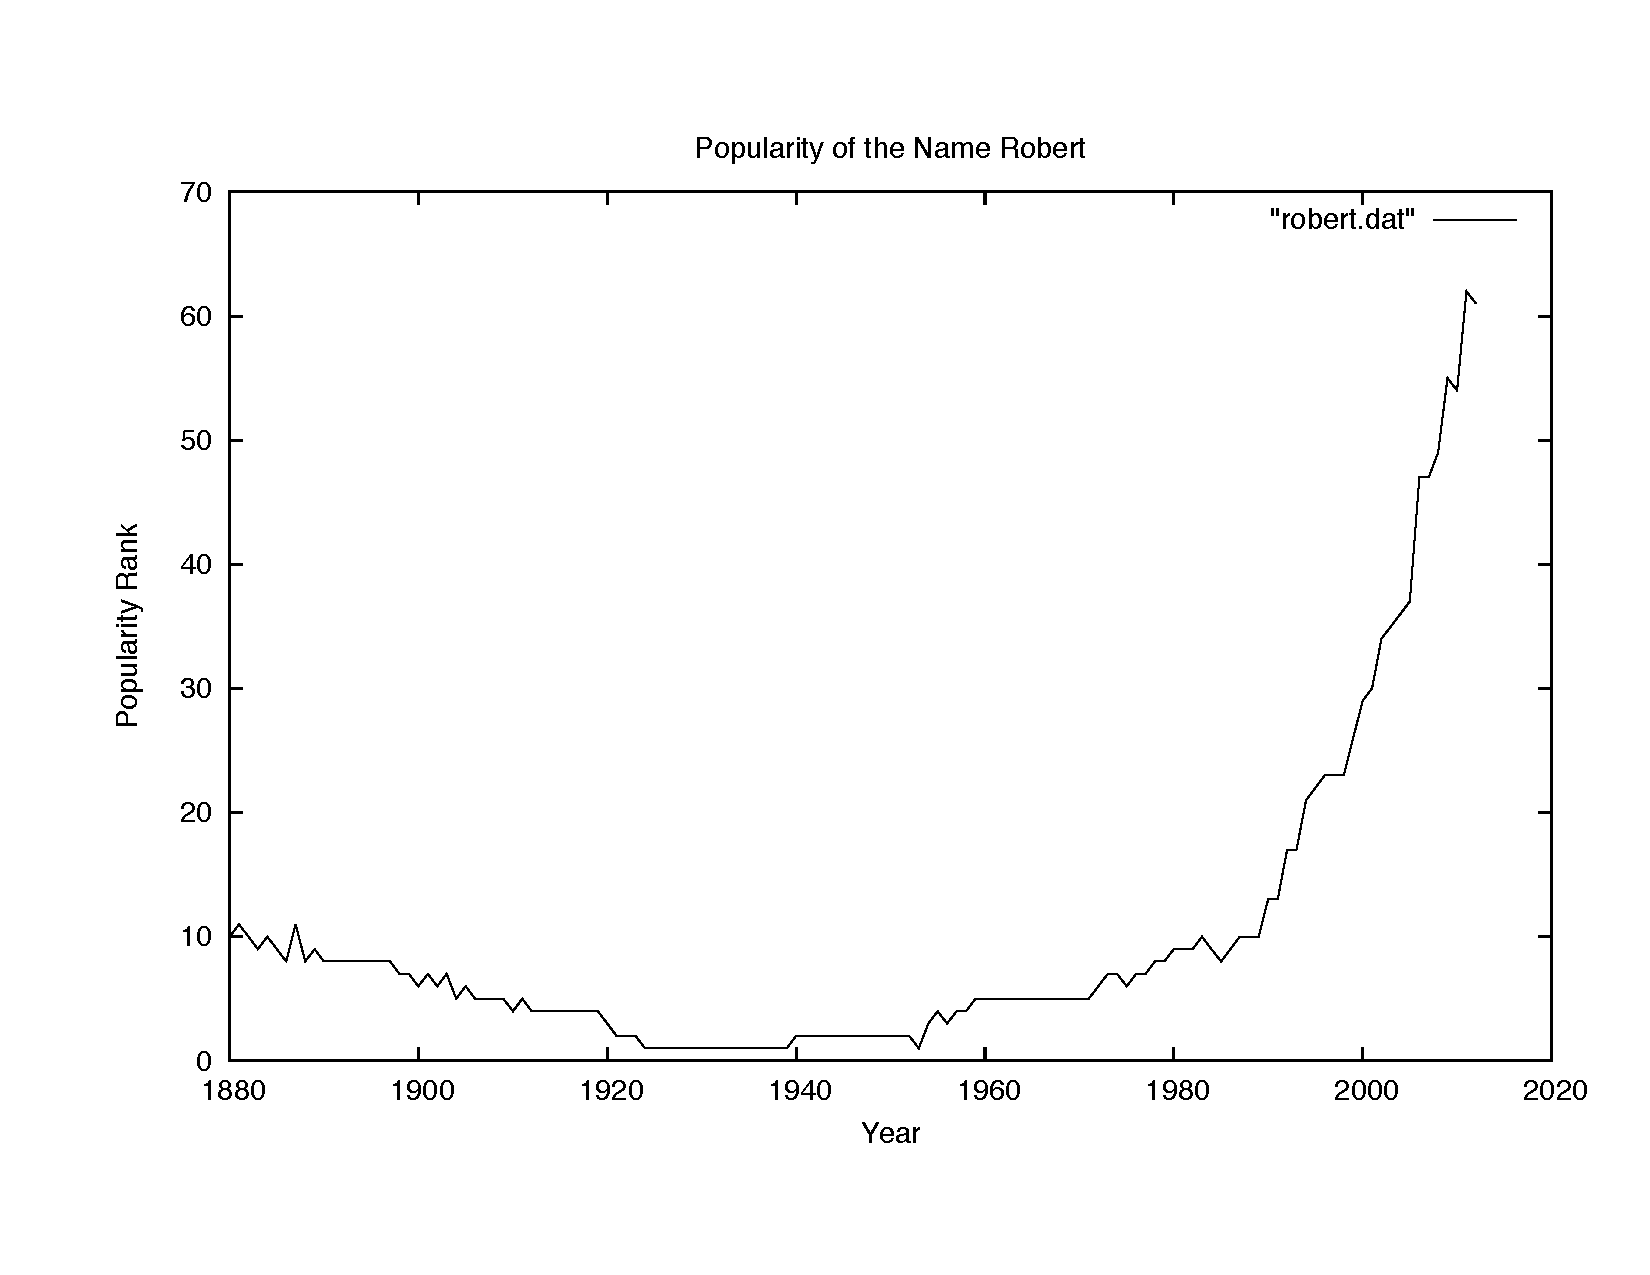
\includegraphics[width=0.8\hsize]{art/robertyears}
    \end{center}
\end{frame}

%------------------------------------------------

\begin{frame}
	\frametitle{Body Mass Index}
	\begin{itemize}
        \item $BMI = \frac{mass(kg)}{height(m)^2}$
        \item<2-> If you're too dumb to use the metric system, try this:
            $BMI = \frac{mass(lb)}{height(in)^2}\times703.06957964$
        \item<3-> Re-named (from Quetelet index) by Ancel Keys.
        \item<4-> Makes sense if you sell insurance, but widely misused today.
    \end{itemize}
\end{frame}

%------------------------------------------------

\begin{frame}
	\frametitle{Magn\'{u}s Ver Magn\'{u}sson: A Severely Obese Man}
	\begin{center}
        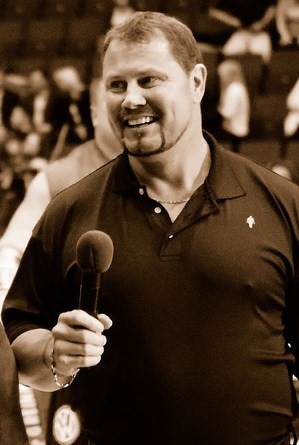
\includegraphics[width=0.3\hsize]{art/magnus}
    \end{center}
    BMI=36
\end{frame}

%------------------------------------------------

\section{Through Thick and Thin}
\begin{frame}
	\frametitle{Know Your Customer}
	\begin{itemize}
        \item Target collects and buys a large amount of data about their customers.
        \item In 2002, they had a statistician predict habit changing queues.
        \begin{itemize}
            \item<2-> New parents spend a lot of money.
            \item<2-> Target sells a wide variety of products.
            \item<2-> A busy person for time might buy \emph{everything} at Target.
        \end{itemize}
    \end{itemize}
\end{frame}

%------------------------------------------------

\begin{frame}
	\frametitle{Bullseye!}
	\begin{itemize}
        \item<1-> In 2012, a teenager in MN received coupons for a crib, baby cloths, and diapers.
        \item<2-> Her father went to the store to complain.
        \item<3-> He later found out that his daughter actually was pregnant.
        \item<4-> Target later changed their policy:
        \begin{itemize}
            \item<4-> Used split testing to identify less-creepy adverts.
            \item<4-> No ``baby specific'' coupon books.
            \item<4-> Diaper coupons next to a lawnmower coupon.
        \end{itemize}
        \item<5->\textbf{Takeaway:}  Don't let on how much you know.
    \end{itemize}
\end{frame}

%------------------------------------------------

\section{Pandora's Box}
\begin{frame}
	\frametitle{Google Flu}
    \begin{center}
        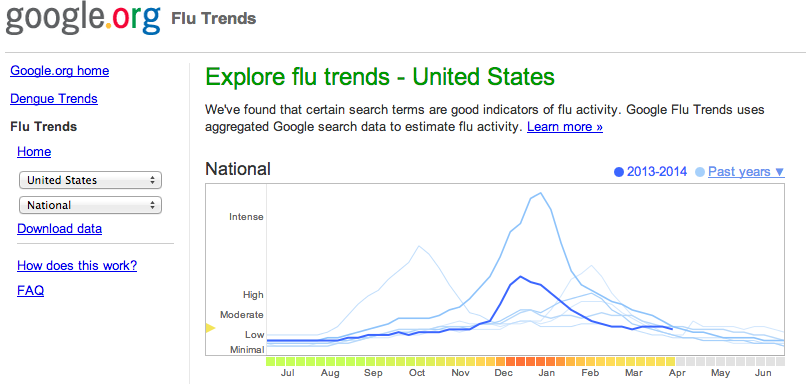
\includegraphics[width=0.9\hsize]{art/google_flu}
    \end{center}
\end{frame}

%------------------------------------------------

\begin{frame}
\frametitle{Google Flu}
    \begin{itemize}
        \item Published in Nature in 2008.\footnote{
            \textit{Detecting influenza epidemics using search engine
            query data}, Ginsberg, et al, Nature 457, 1012-1014 (19 February
            2009)}
        \item<2-> Took 1152 CDC data points, searched for correlated searches.
        \item<3-> Manually filtered unrelated terms (e.g., basketball).
        \item<4-> Predicts flu pandemics 2 weeks faster than CDC stats.
    \end{itemize}
    \begin{center}
        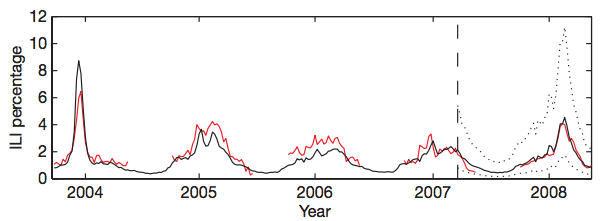
\includegraphics[width=0.8\hsize]{art/googleflugraph}
    \end{center}
\end{frame}

%------------------------------------------------

\begin{frame}
    \frametitle{Google Flu}
    \begin{itemize}
        \item Except that it had to be updated in 2009, and it stopped working in 2010, 2011, and 2012.
        \item Off by a factor of 2.
        \item<2->Critical study published in Science in March 2014.\footnote{\textit{The Parable of Google 
            Flu: Traps in Big Data Analysis}, Lazer et al, Science 14 March
            2014: Vol. 343 no. 6176 pp. 1203-1205}
        \item<3->Accuracy was not much better than a projection using already available CDC data.
    \end{itemize}
\end{frame}

%------------------------------------------------

\section{Conclusion}
\begin{frame}
	\frametitle{Conclusion}
	\begin{itemize}
        \item<1->Are you just making an observation?
        \item<2->Do you just want to make money on average?
        \item<3->Do not misuse statistics.  Consult a textbook.
        \item<4->Make sure your data captures the thing you are interested in.
        \item<5->Thick vs thin data.
        \item<6->Do not discount human responses to your result.
    \end{itemize}
\end{frame}

%------------------------------------------------

\begin{frame}
\frametitle{Thank You}
\begin{itemize}
    \item Thank you for your time and attention.
    \item rob.lass@gmail.com
    \item github.com/roblass
    \item @therealroblass
    \item Questions?
\end{itemize}
\end{frame}
\end{document}
